\documentclass[journal]{IEEEtran}
\usepackage[english]{babel}

\usepackage{amssymb, amsmath} %Paquetes matemáticos de la American Mathematical 
\usepackage[utf8]{inputenc}
\usepackage{graphicx}
\usepackage{float}
\usepackage{hyperref}
\usepackage{listings}
\usepackage{xcolor}

\definecolor{codegreen}{rgb}{0,0.6,0}
\definecolor{codegray}{rgb}{0.5,0.5,0.5}
\definecolor{codepurple}{rgb}{0.58,0,0.82}
\definecolor{backcolour}{rgb}{0.95,0.95,0.92}
% Definicio de estilo para el codigo fuente que se cita
\lstdefinestyle{mystyle}{
    backgroundcolor=\color{backcolour},   
    commentstyle=\color{codegreen},
    keywordstyle=\color{magenta},
    numberstyle=\tiny\color{codegray},
    stringstyle=\color{codepurple},
    basicstyle=\ttfamily\footnotesize,
    breakatwhitespace=false,         
    breaklines=true,                 
    captionpos=b,                    
    keepspaces=true,
    numbers=left,                    
    numbersep=5pt,                  
    showspaces=false,                
    showstringspaces=false,
    showtabs=false,                  
    tabsize=2,
}
\lstset{style=mystyle}

\renewcommand{\lstlistingname}{Código}

\ifCLASSINFOpdf

\else

\fi
\begin{document}

\title{Ejercicio 6 - tema 6 \\ Administración de espacio asignado a un tablespace}
%
\author{Vicente Romero Andrade}

\markboth{Ejercicio 6 - tema 6 Administración de espacio asignado a un tablespace, Julio~2021}%
{Shell \MakeLowercase{\textit{et al.}}: }
% The only time the second header will appear is for the odd numbered pages

\maketitle


\IEEEpeerreviewmaketitle

\section{Objetivo}
% The very first letter is a 2 line initial drop letter followed

\IEEEPARstart{E}{l} objetivo es comprender y poner en práctica las diferentes opciones que existen 
para modificar la capacidad de almacenamiento de un tablespace
\section{Desarrollo}
\subsection{sentencias}
\begin{lstlisting}[language=sql, caption=s-00-tablespaces.sql,label={lst:codigo1}]
  whenever sqlerror continue
set serveroutput on
connect store_user/store_user
--A
declare
  v_count number;
  v_username varchar2(30) := 'STORE_USER';
  v_table varchar2(30) := 'TEST';
begin
  --Verificar si la table existe
  select count(*) into v_count
  from all_tables
  where table_name = v_table
  and owner = v_username;
  --Si existe la tabla, entonces se borra
  if v_count > 0 then
    execute immediate 'drop table '||v_table;
  end if;
  execute immediate 'create table '||v_table||' (
    id number,
    nombre varchar(200),
    apellido varchar(200)
  ) segment creation deferred';
end;
/

--B
declare
  v_count number := 0;
begin
  --Verificar si la table existe
  while true loop
  v_count := v_count + 1;
  insert into test(id,nombre,apellido) values(v_count,'nombre random','apellido random');
  commit;
  end loop;
end;
/
select
  count(SEGMENT_NAME) NUMERO_EXTENSIONES,
  trunc(SUM(BYTES)/(1024*1024),2) ALLOCATED_MB
from USER_EXTENTS;
--C
connect sys/system2 as sysdba
alter tablespace store_tbs1
add datafile '/u01/app/oracle/oradata/VRABDA2/store_tbs02.dbf' size 5M;
--D
connect store_user/store_user
declare
  v_count number := 0;
begin
  --Verificar si la table existe
  while true loop
    v_count := v_count + 1;
    insert into test(id,nombre,apellido) values(v_count,'nombre random','apellido random');
    commit;
  end loop;
end;
/
select 
  count(SEGMENT_NAME) NUMERO_EXTENSIONES,
  trunc(SUM(BYTES)/(1024*1024),2) ALLOCATED_MB
from USER_EXTENTS;
--E
SELECT distinct t.TABLESPACE_NAME nombre, count(s.TABLESPACE_NAME) numero_segmentos FROM DBA_TABLESPACES t
  left JOIN DBA_SEGMENTS s on t.TABLESPACE_NAME=s.TABLESPACE_NAME
  group by t.TABLESPACE_NAME order by numero_segmentos desc;
\end{lstlisting}
\subsection{Resultados}
\begin{figure}[H]
  \centering
  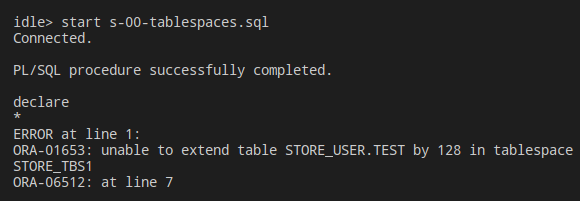
\includegraphics[scale=.30]{captura_1.png}
   \caption{Salida punto B}
   \label{fig:validador_1}
\end{figure}
\begin{figure}[H]
  \centering
  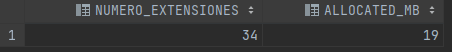
\includegraphics[scale=.30]{captura_2.png}
   \caption{Salida punto B tamaño y extensiones}
   \label{fig:validador_2}
\end{figure}
\begin{figure}[H]
  \centering
  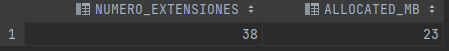
\includegraphics[scale=.30]{captura_4.png}
   \caption{Salida punto C tamaño y extensiones}
   \label{fig:validador_4}
\end{figure}
\begin{figure}[H]
  \centering
  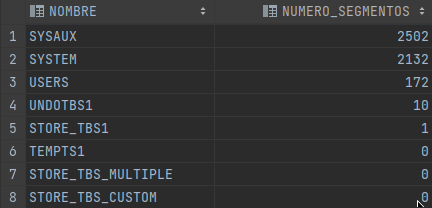
\includegraphics[scale=.30]{captura_3.png}
   \caption{Salida punto E}
   \label{fig:validador_3}
\end{figure}
\section{Conclusiones}
Se logro hacer una administración a nivel base en funcionamiento del espacio de almacenamiento de los tablespace,
fue util ya que esto servira para evitar problemas de un espacio mal planificado.
\ifCLASSOPTIONcaptionsoff
  \newpage

\fi

\end{document}
